\documentclass[convert = false, tikz]{standalone}
\usepackage[utf8]{inputenc}
\usepackage{tikz}
\usetikzlibrary{automata, positioning, arrows}
 
\usepackage{../../../../style_automata}

% arara: pdflatex
% arara: latexmk: { clean: partial }
\begin{document}
    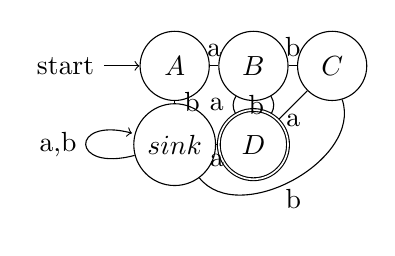
\begin{tikzpicture}
        \node[state, initial] (a) {$A$};
        \node[state, right of=a] (b) {$B$};
        \node[state, right of=b] (c) {$C$};
        \node[state, below of=a] (sink) {$sink$};
        \node[state, accepting, below of=b] (d) {$D$};
	    \draw (a) edge[above] node{a} (b)
        (a) edge[right] node{b} (sink)
        (b) edge[above] node{b} (c)
        (b) edge[left, bend right=30] node{a} (d)
        (c) edge[below] node{a} (d)
        (c) edge[below, bend left=80] node{b} (sink)
        (d) edge[left, bend right=30] node{b} (b)
        (d) edge[below] node{a} (sink)
        (sink) edge[loop left] node{a,b} (sink);
    \end{tikzpicture}
\end{document}
